\section{CAN-Bus}
CAN steht für Controller Area Network und gehört zu den Feldbussystemen. Dieses Feldbussystem findet zahlreiche Anwendungsmöglichkeiten unter anderem in der Automobilindustrie, Automatisierungstechnik und in vielen weiteren Bereichen. In dieser Arbeit wurde der Feldbus verwendet, um mit dem BLDC-Motor zu kommunizieren. 

\subsection{Funktionsweise}
Bei CAN-Bus Systemen sind mehrere gleichrangige Steuerelemente miteinander verbunden, dieses Prinzip hei{\ss}t „Multi-Master-Prinzip“. Um Kollisionen zu lösen, wird das CSMA/CR-Verfahren eingesetzt, dazu muss es verschieden hochrangige Zustände geben. Bei diesem System hat die logische 0 eine höhere Priorität und wird bei einer Kollision somit übertragen. Wenn der CAN-Bus mit Kupferleitungen arbeitet, werden zwei Adern miteinander verdrillt, diese fungieren als CAN HIGH (CAN\_H) und CAN LOW (CAN\_L) und haben verschieden hohe Spannungspotenziale (z.B.: CAN\_H: 5V und CAN\_L: 3V). Diesen Vorgang wird NRZ-Bitcodierung (Non Return to Zero) genannt. Somit werden die Eigenschaften der symmetrischen Signalübertragung genutzt, um Störungen minimal zu halten bzw. ganz auszulöschen. Je höher die Übertragungsrate sein soll, desto niedriger muss die Spannungsdifferenz zwischen CAN HIGH und CAN LOW sein und desto niedriger ist die maximale Reichweite. 

\clearpage

\subsubsection{Multimaster Prinzip}
Bei dem Multimaster Prinzip gibt es mehrere Master, die über ein Gateway miteinander kommunizieren können. \\
Das kann so wie in Abbildung 6 aussehen. \\

\begin{figure}[h]
    \begin{center}
        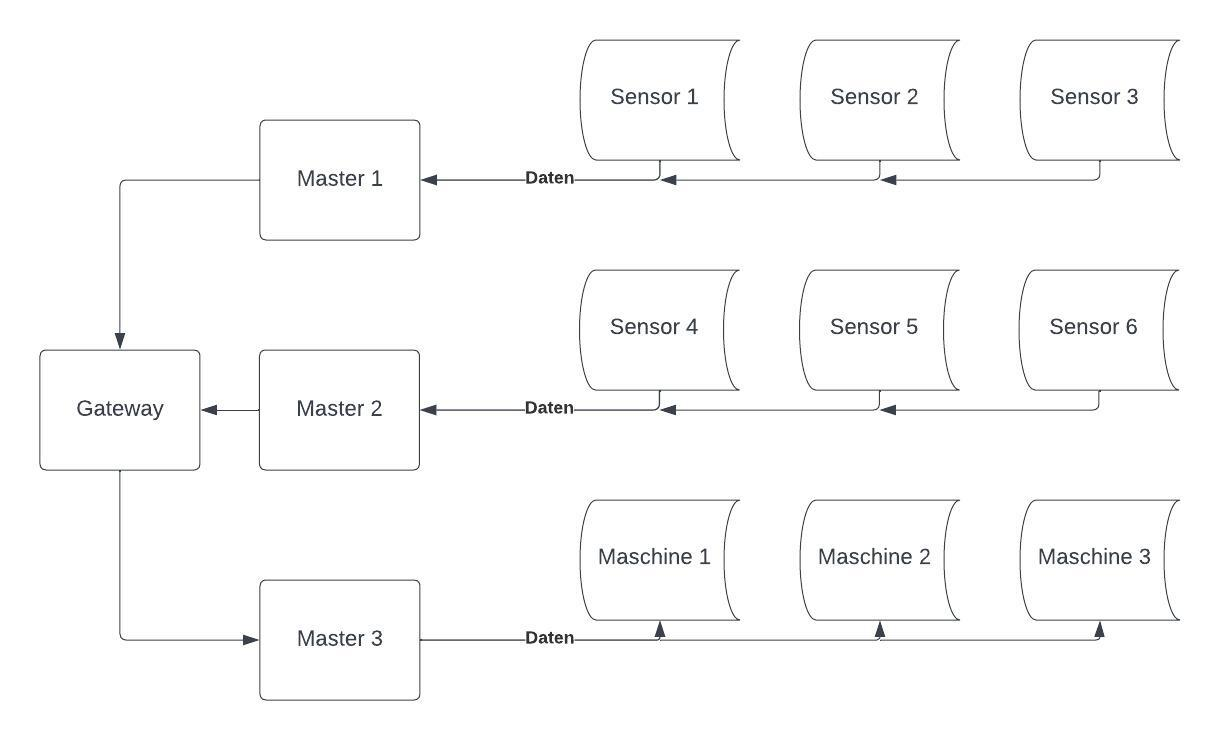
\includegraphics[width=13.98cm, height= 8.48cm]{images/Abbildung 6.jpeg}
        \caption{Multimaster Prinzip}
        \label{MMaster}
        \end{center}
\end{figure}

In diesem Beispiel senden Master eins und zwei Daten, die sie von den Sensoren erhalten, Master drei verarbeitet diese Daten und steuert damit seine Maschinen. Bei diesem Prinzip ist es möglich das zwei Master gleichzeitig senden und es somit zu einer Kollision kommt. Welcher von beiden seine Nachricht durchführen darf, wird nach dem CSMA/CR Protokoll entschieden. 

\clearpage
\subsubsection{CSMA/CR}
Carrier Sense Multiple Access / Collision Resolution funktioniert aufgrund von Bitarbitrierung. Ein Bitarbitrierer ist eine Schaltung, die möglichst schnell entscheiden kann, welches von beiden gesendeten Signalen eine höhere Priorität hat. Eine Kollision wird also erkannt, und dann anders wie bei CSMA/CA nicht abgewartet, sondern entschieden welches von den beiden Signalen den freien Sendeplatz bekommt. In Abbildung 7 ist dieser Verlauf verbildlicht. \\

\begin{figure}[h]
    \begin{center}
        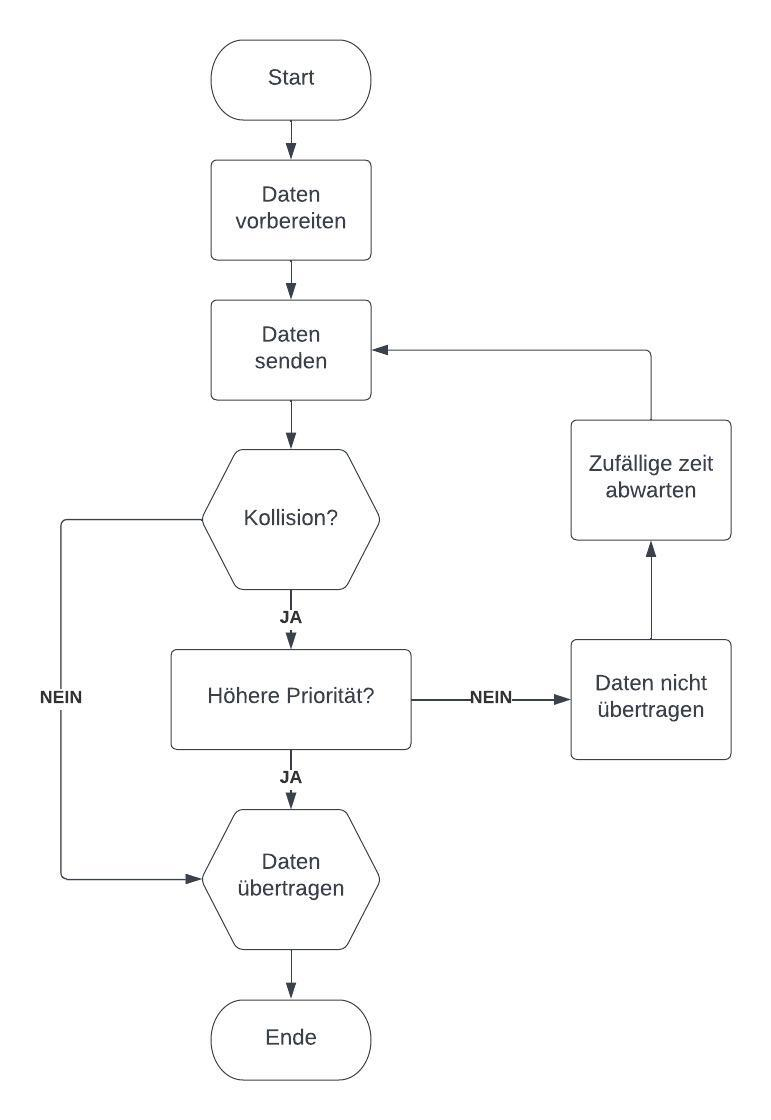
\includegraphics[width=12.24cm, height= 17.78cm]{images/Abbildung 7.jpeg}
        \caption{CSMA/CR Flussdiagramm}
        \label{CSMA/CR}
        \end{center}
\end{figure}

\clearpage

\subsubsection{Non Return to Zero (NRZ-Bitcodierung)}
Die NRZ-Bitcodierung wurde für CAN-Bussysteme gewählt, denn diese Art von Codierung erlaubt hohe Datenraten mit sehr geringen Verlusten. In diesem Fall gibt es keinen Leiter mit einem Null-Potential, ein dominantes Bit wird durch ein hohen Potenzialunterschied und ein rezessives Bit wird durch einen niedrigen Potenzialunterschied dargestellt. In Abbildung 8 ist das an einem Beispiel von Highspeed-CAN verbildlicht. \\

\begin{figure}[h]
    \begin{center}
        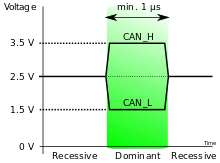
\includegraphics[width=8.66cm, height=6.39cm]{images/Abbildung 8.png}
        \caption{Spannungsdifferenz im Highspeed-CAN}
        \label{Highspeed-CAN}
        \end{center}
\end{figure}
Ein Nachteil dieser Bitcodierung ist, dass der Empfänger die Synchronisation verliert, wenn der Pegel lange unverändert bleibt. Die Lösung zu diesem Problem nennt sich Bitstuffing. Dieser Synchronisierungsmechanismus sendet nach fünf homogenen Bits ein komplementäres Bit, dass dem Empfänger den Takt vorgibt. \\

\subsection{Topologie}
Der Aufbau von CAN-Bus Systemen ist meist einer Linie entlang strukturiert, es gibt auch sternförmige Topologien, diese haben im Vergleich jedoch Nachteile. Da sternförmige Aufbauten meist über einen Hauptrechner laufen, kommt es beim Ausfall von diesem zu einem kompletten Ausfall des Systems. Bei der häufigsten Art kann es nur bei einem Ausfall der Adern zu einem Komplettausfall kommen. \\

\begin{figure}[h]
    \begin{center}
        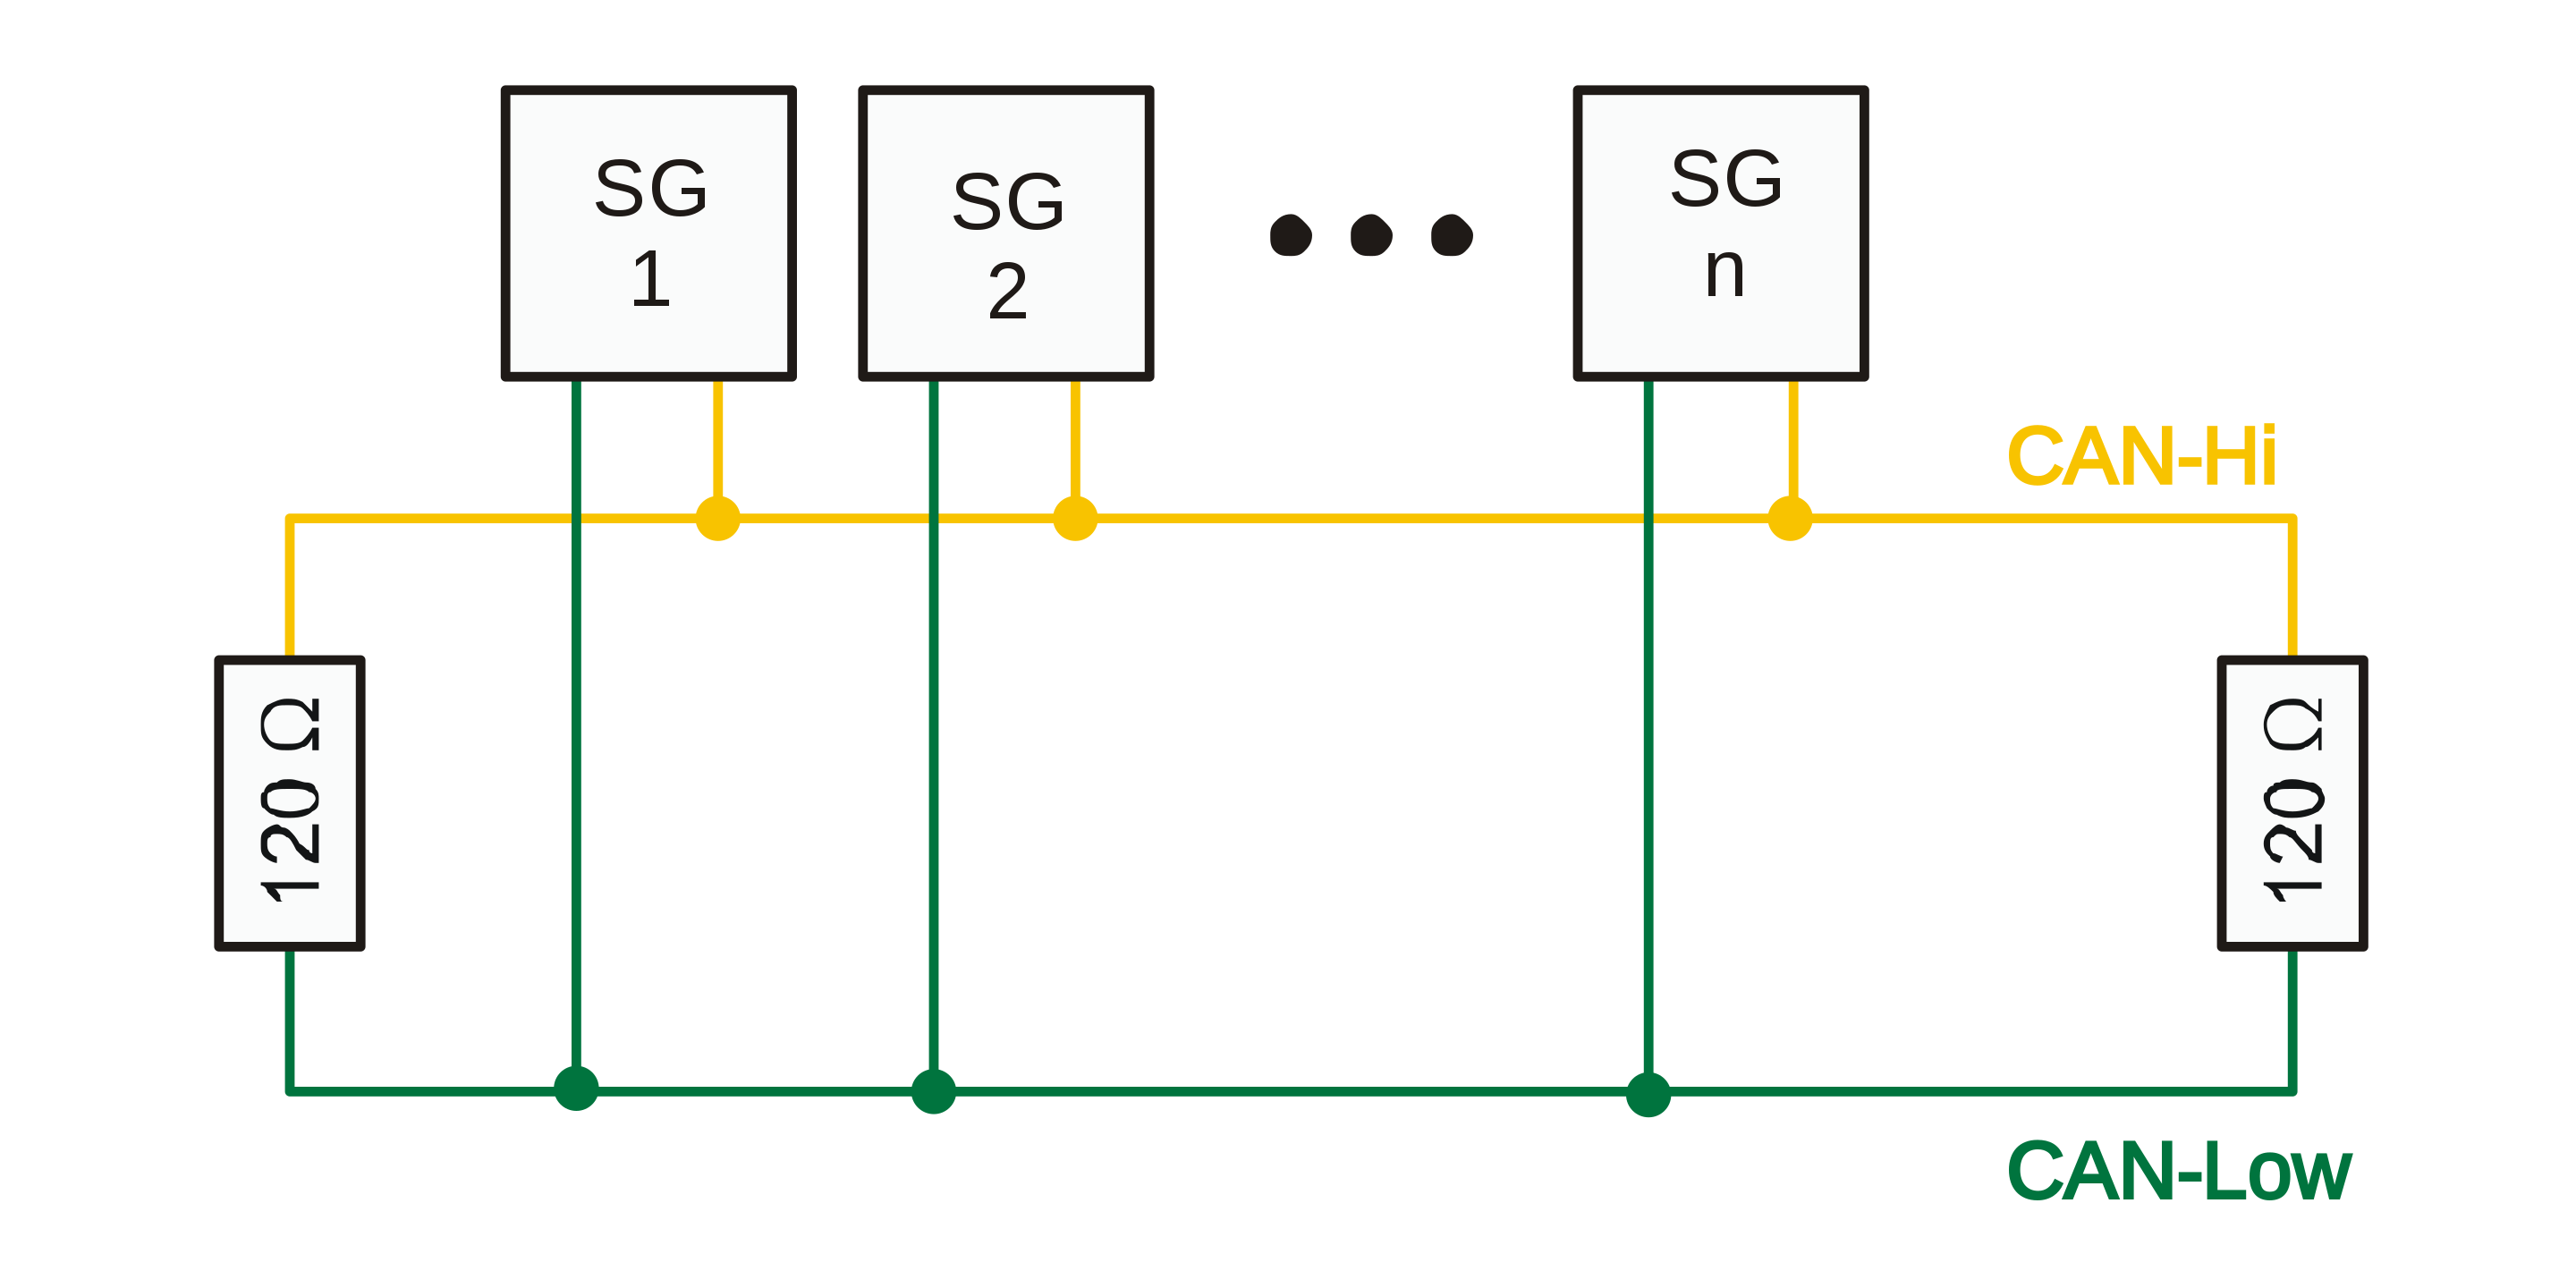
\includegraphics[width=10.08cm, height=5.04cm]{images/Abbildung 9.png}
        \caption{CAN-Bus in Linientopologie}
        \label{Linientopologie}
        \end{center}
\end{figure}
Die Abschlusswiderstände von 120 Ohm sind vorhanden, um Reflexionen zu vermeiden. Eine Reflexion von Wellen ist die Überlagerung von einer zurücklaufenden Welle und einer vorlaufenden Welle, dass bildet eine stehende Welle auf der Leitung und beeinflusst das Signal. 

\clearpage

\subsection{Anwendungsbereiche}
